\documentclass[conference]{IEEEtran}
\IEEEoverridecommandlockouts
% The preceding line is only needed to identify funding in the first footnote. If that is unneeded, please comment it out.
\usepackage{cite}
\usepackage{amsmath,amssymb,amsfonts}
\usepackage{algorithmic}
\usepackage{graphicx}
\usepackage{textcomp}
\usepackage{xcolor}
\usepackage{multirow}
\usepackage{caption}
\usepackage{subcaption}
\usepackage{pgfplots}
\usepackage{makecell}
\usepackage{pgfplotstable}





\def\BibTeX{{\rm B\kern-.05em{\sc i\kern-.025em b}\kern-.08em
    T\kern-.1667em\lower.7ex\hbox{E}\kern-.125emX}}
\begin{document}

\title{Emergency Vehicle Traffic Signal Control\\
{\footnotesize \textsuperscript{}}
\thanks{}
}

\author{\IEEEauthorblockN{1\textsuperscript{st} Dr. C. Gomathy}
\IEEEauthorblockA{\textit{VP and Professor/ECE} \\
\textit{SRMIST, Vadapalani}\\
vp.academics.vdp@srmist.edu.in     }
\and
\IEEEauthorblockN{2\textsuperscript{nd}      Anushka Prasad}
\IEEEauthorblockA{\textit{Student/ECE} \\
\textit{SRMIST, Vadapalani)} \\
ap9802@srmist.edu.in}
\and
\IEEEauthorblockN{3\textsuperscript{rd} Parvatha Varshini LS}
\IEEEauthorblockA{\textit{Student/ECE} \\
\textit{SRMIST, Vadapalani}\\
pl9041@srmist.edu.in}
\and
\IEEEauthorblockN{\textsuperscript{} }
\IEEEauthorblockA{\textit{} \\
\textit{}\\
\\}
\and
\IEEEauthorblockN{\textsuperscript{} }
\IEEEauthorblockA{\textit{} \\
\textit{}\\
\\
}
\and
\IEEEauthorblockN{\textsuperscript{} }
\IEEEauthorblockA{\textit{} \\
\textit{}\\
\\
}
}

\maketitle

\begin{abstract}
This project presents a Emergency Vehicle Traffic Signal Control System aimed at improving emergency response times for emergency vehicles like ambulances and firetrucks in urban traffic. By integrating a sound sensor and an ESP32 camera, the system detects the unique frequency of ambulance sirens and visually verifies the vehicle's presence. A dual-confirmation mechanism ensures that both sound and visual cues must align before the traffic light is switched to green, minimizing false activations. Upon confirmation, the system overrides the standard traffic light cycle, allowing the ambulance to pass without delay. Testing demonstrated a reliability rate of approximately 95 percentage and a response time of less than one second. This innovative solution enhances public safety and traffic efficiency, showcasing the potential of IoT technologies in smart city initiatives.
\end{abstract}

\begin{IEEEkeywords}
ESP32 Cam, Sound Sensor, Traffic Signal Control, Image and Sound Detection, iot, Real-time monitoring
\end{IEEEkeywords}



\section{Introduction}
The rapid movement of emergency vehicles, such as ambulances and firetrucks is critical for timely assistance in life-threatening situations. Delays caused by conventional traffic systems, especially in urban areas, can hinder the response time of these vehicles, directly impacting life-threatening situations and its outcomes. Traditional traffic control systems lack mechanisms to recognize and prioritize emergency vehicles dynamically. Consequently, there is an urgent need for innovative solutions that integrate real-time response capabilities into traffic management systems to minimize delays for emergency vehicles.

The "Emergency Vehicle Traffic Control System" addresses this issue by employing an intelligent traffic control approach, which combines image and sound recognition technologies to identify ambulances. Leveraging components like the ESP32-CAM, Arduino microcontrollers, and Python programming, this system effectively identifies an ambulance based on both visual and audio cues. Once an ambulance is detected, the system overrides the regular traffic light cycle to provide a green signal, facilitating an unhindered passage. This innovative approach aims to enhance road safety and efficiency, addressing the limitations of static traffic control systems.

In the proposed system, the ESP32-CAM module captures real-time images of the traffic, while sound detection sensors monitor the unique siren patterns of emergency vehicles. This dual-detection method enhances the system's accuracy, robustness, and practical applicability in various traffic conditions. The traffic signal board's red and green light changes are central to the system's functionality. When an ambulance is detected, the system overrides the usual traffic light sequence, switching the light to green in the ambulance’s direction to ensure a clear path.

\section{Related Works}
Some of the notable research papers and studies on emergency vehicle prioritization and smart traffic systems, along with details on their authors and key contributions: 
A study by Chen, Liu, and Wang(2018) [1]“Traffic Signal Preemption Strategy for Emergency Vehicles Using V2I Communication". This study by researchers at Tsinghua University explored the use of Vehicle-to-Infrastructure (V2I) communication to improve emergency response times. The authors proposed a system where emergency vehicles communicate with traffic signals via V2I to clear intersections. The research demonstrated a reduction in response time but noted limitations in regions without extensive V2I infrastructure. Source: IEEE Transactions on Intelligent Transportation Systems. Another research by Sharma, Patil, and Gupta in 2019[2] ”A Smart Traffic Signal System for Emergency Vehicle Priority and Traffic Congestion Control Using IoT" along with researchers from the Indian Institute of Technology developed a system that uses IoT and cloud-based data processing to manage traffic for emergency vehicles. By deploying sensors and cameras, the system collects real-time data on traffic density and prioritizes emergency vehicles at intersections. This study highlighted the potential for IoT in real-time traffic control but noted challenges in data transmission latency. Source: International Journal of Innovative Technology and Exploring Engineering (IJITEE). Looking at another research done by the researchers from Seoul National University ie., Kim, Lee, and Park(2020)[3]”Emergency Vehicle Detection Using Acoustic Sensors and Deep Learning" presented a sound-based detection method using deep learning to identify emergency vehicle sirens. Their model, trained on sound frequency patterns, achieved high accuracy in distinguishing emergency sirens from background noise. This approach showed promise, though the authors noted that it struggled with high urban noise and extreme weather conditions. Source: IEEE Access. [4]”Intelligent Traffic Light Control System for Emergency Vehicle Preemption Using RFID Technology" by Alotaibi and Mehmood(2017): This study by Alotaibi and Mehmood from King Saud University examined RFID-based traffic preemption for emergency vehicles. By attaching RFID tags to emergency vehicles and readers to intersections, the system prioritized emergency vehicle passage. While effective, the study highlighted the limitations of RFID, such as its dependency on direct line-of-sight and limited range. Source: Procedia Computer Science. [5]”Vision-Based Real-Time Traffic Signal Control System for Emergency Vehicles Using Deep Learning" by Jain, Aggarwal, and Kumar(2021). Researchers from Delhi University applied deep learning models to image data from cameras to detect emergency vehicles visually. Using Convolutional Neural Networks (CNNs), the system identifies emergency vehicles and prioritizes them by adjusting traffic signals. Their approach yielded high accuracy but required high-quality cameras and extensive data processing power. Source: Journal of Computer Vision and Image Processing.[6]“Evaluation of Adaptive Traffic Signal Control for Emergency Vehicle Preemption Using Reinforcement Learning" by Xu, Zhang, and Chen (2022). This study from Peking University introduced reinforcement learning for adaptive traffic signal control. The system learned from traffic patterns and prioritized emergency vehicles based on real-time data from connected sensors. By applying machine learning to historical data, the system improved over time in predicting and adjusting to emergency situations. Source: Transportation Research Part C: Emerging Technologies.
These studies contribute foundational insights into traffic control technologies, covering a range of methods from RFID and acoustic detection to IoT and machine learning. Each has provided a unique approach to enhancing emergency vehicle prioritization, though most approaches require significant infrastructure investment.

\begin{figure}[htbp]
    \centering 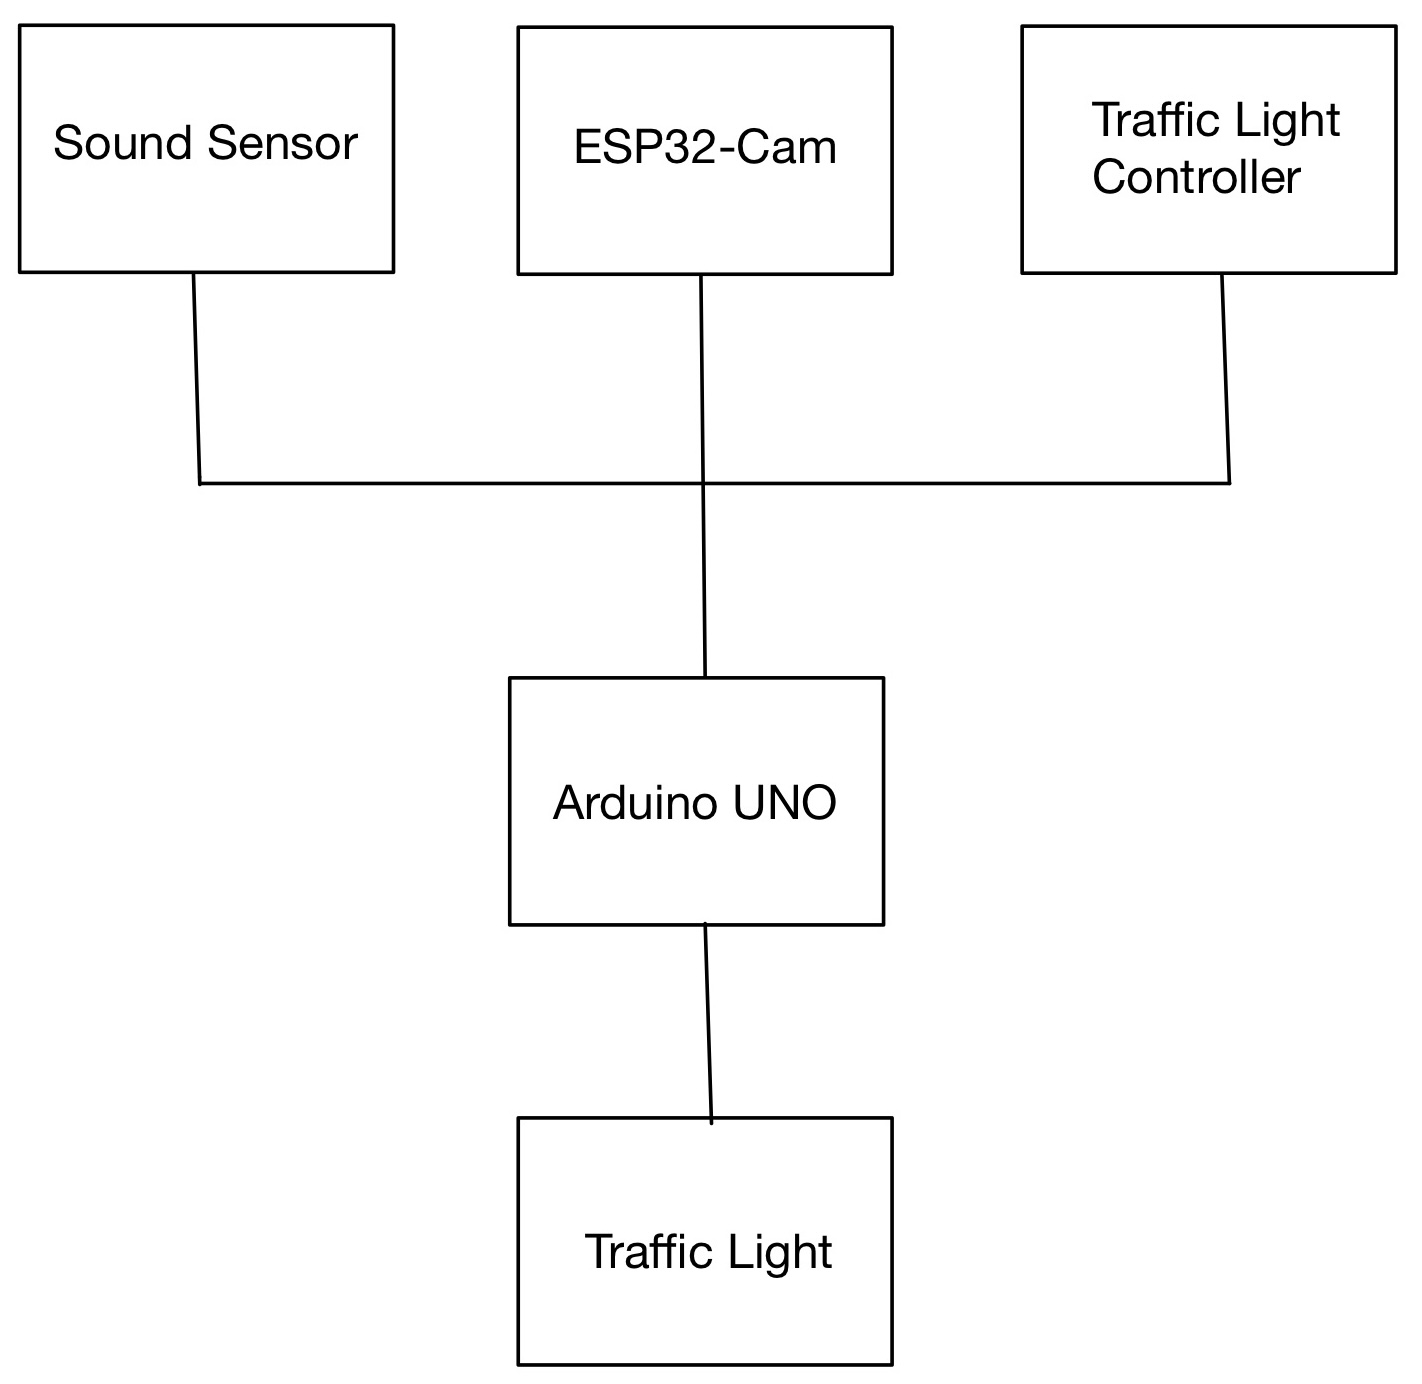
\includegraphics[width=1\linewidth]{block diagram.jpg}
    \caption{Block Diagram}
    \label{fig:enter-label}
\end{figure}


\section{Proposed Model}\label{AA}
Sound detection process involves:
Analog to Digital Conversion: The Arduino converts the analog sound signal to a digital format, allowing it to process and analyze sound levels.
Frequency Analysis: The Arduino detects frequencies typical of ambulance sirens (500–2,000 Hz) and analyzes repeating patterns to distinguish sirens from background noise.
Pattern Recognition: Using pattern recognition, the system checks the modulation, frequency consistency, and repetition to match typical siren patterns.
Response Time: This detection process takes 4–7 seconds, allowing the system to verify the siren sound accurately without delay, ensuring reliable activation.

The visual detection process for the emergency Vehicle traffic light system uses an ESP32-Cam to identify ambulances at intersections, providing visual confirmation to enhance detection accuracy.
Continuous Scanning: The ESP32-Cam continuously captures images, monitoring the intersection for vehicles.
Ambulance Detection Parameters: It looks for ambulance-specific features, like the vehicle’s rectangular shape, color schemes, markings, and emergency lights.
Object Recognition: The camera uses detection algorithms to identify ambulance characteristics, with options for advanced techniques like CNNs to improve accuracy.
Image Processing: Captured images undergo gray scale conversion, edge detection, and feature matching to isolate and identify the ambulance.
Matching with Predefined Criteria: The system compares detected features against predefined ambulance attributes, confirming the vehicle type if there's a strong match.
Response Time: Detection typically takes between 500 milliseconds to 5 seconds, depending on algorithm complexity and environmental conditions like lighting and movement.


The Dual Confirmation of Ambulance Presence is essential for the emergency traffic light system, reducing false positives by requiring both sound and visual verification before activating the green light.
Dual Confirmation Logic: The Arduino integrates both signals, activating the green light only if both sound and visual confirmations are present.
Timing Considerations: The system synchronizes inputs from both sensors at regular intervals, ensuring timely and accurate response without unnecessary delays.

The Traffic Light Control Mechanism changes the regular cycle to prioritize ambulance movement. Once the ambulance is confirmed through sound and visual detection, the Arduino immediately switches the traffic light to green for the ambulance’s lane, bypassing the typical red-yellow-green sequence. It overrides any red or yellow light, ensuring no delay. The system controls each lane's traffic lights via specific pins, activating only the ambulance's path. This quick transition reduces delays, improves safety, and eliminates manual intervention. After a preset duration, the system reverts to the normal traffic cycle, restoring regular traffic flow.

\begin{figure}[htbp]
    \centering 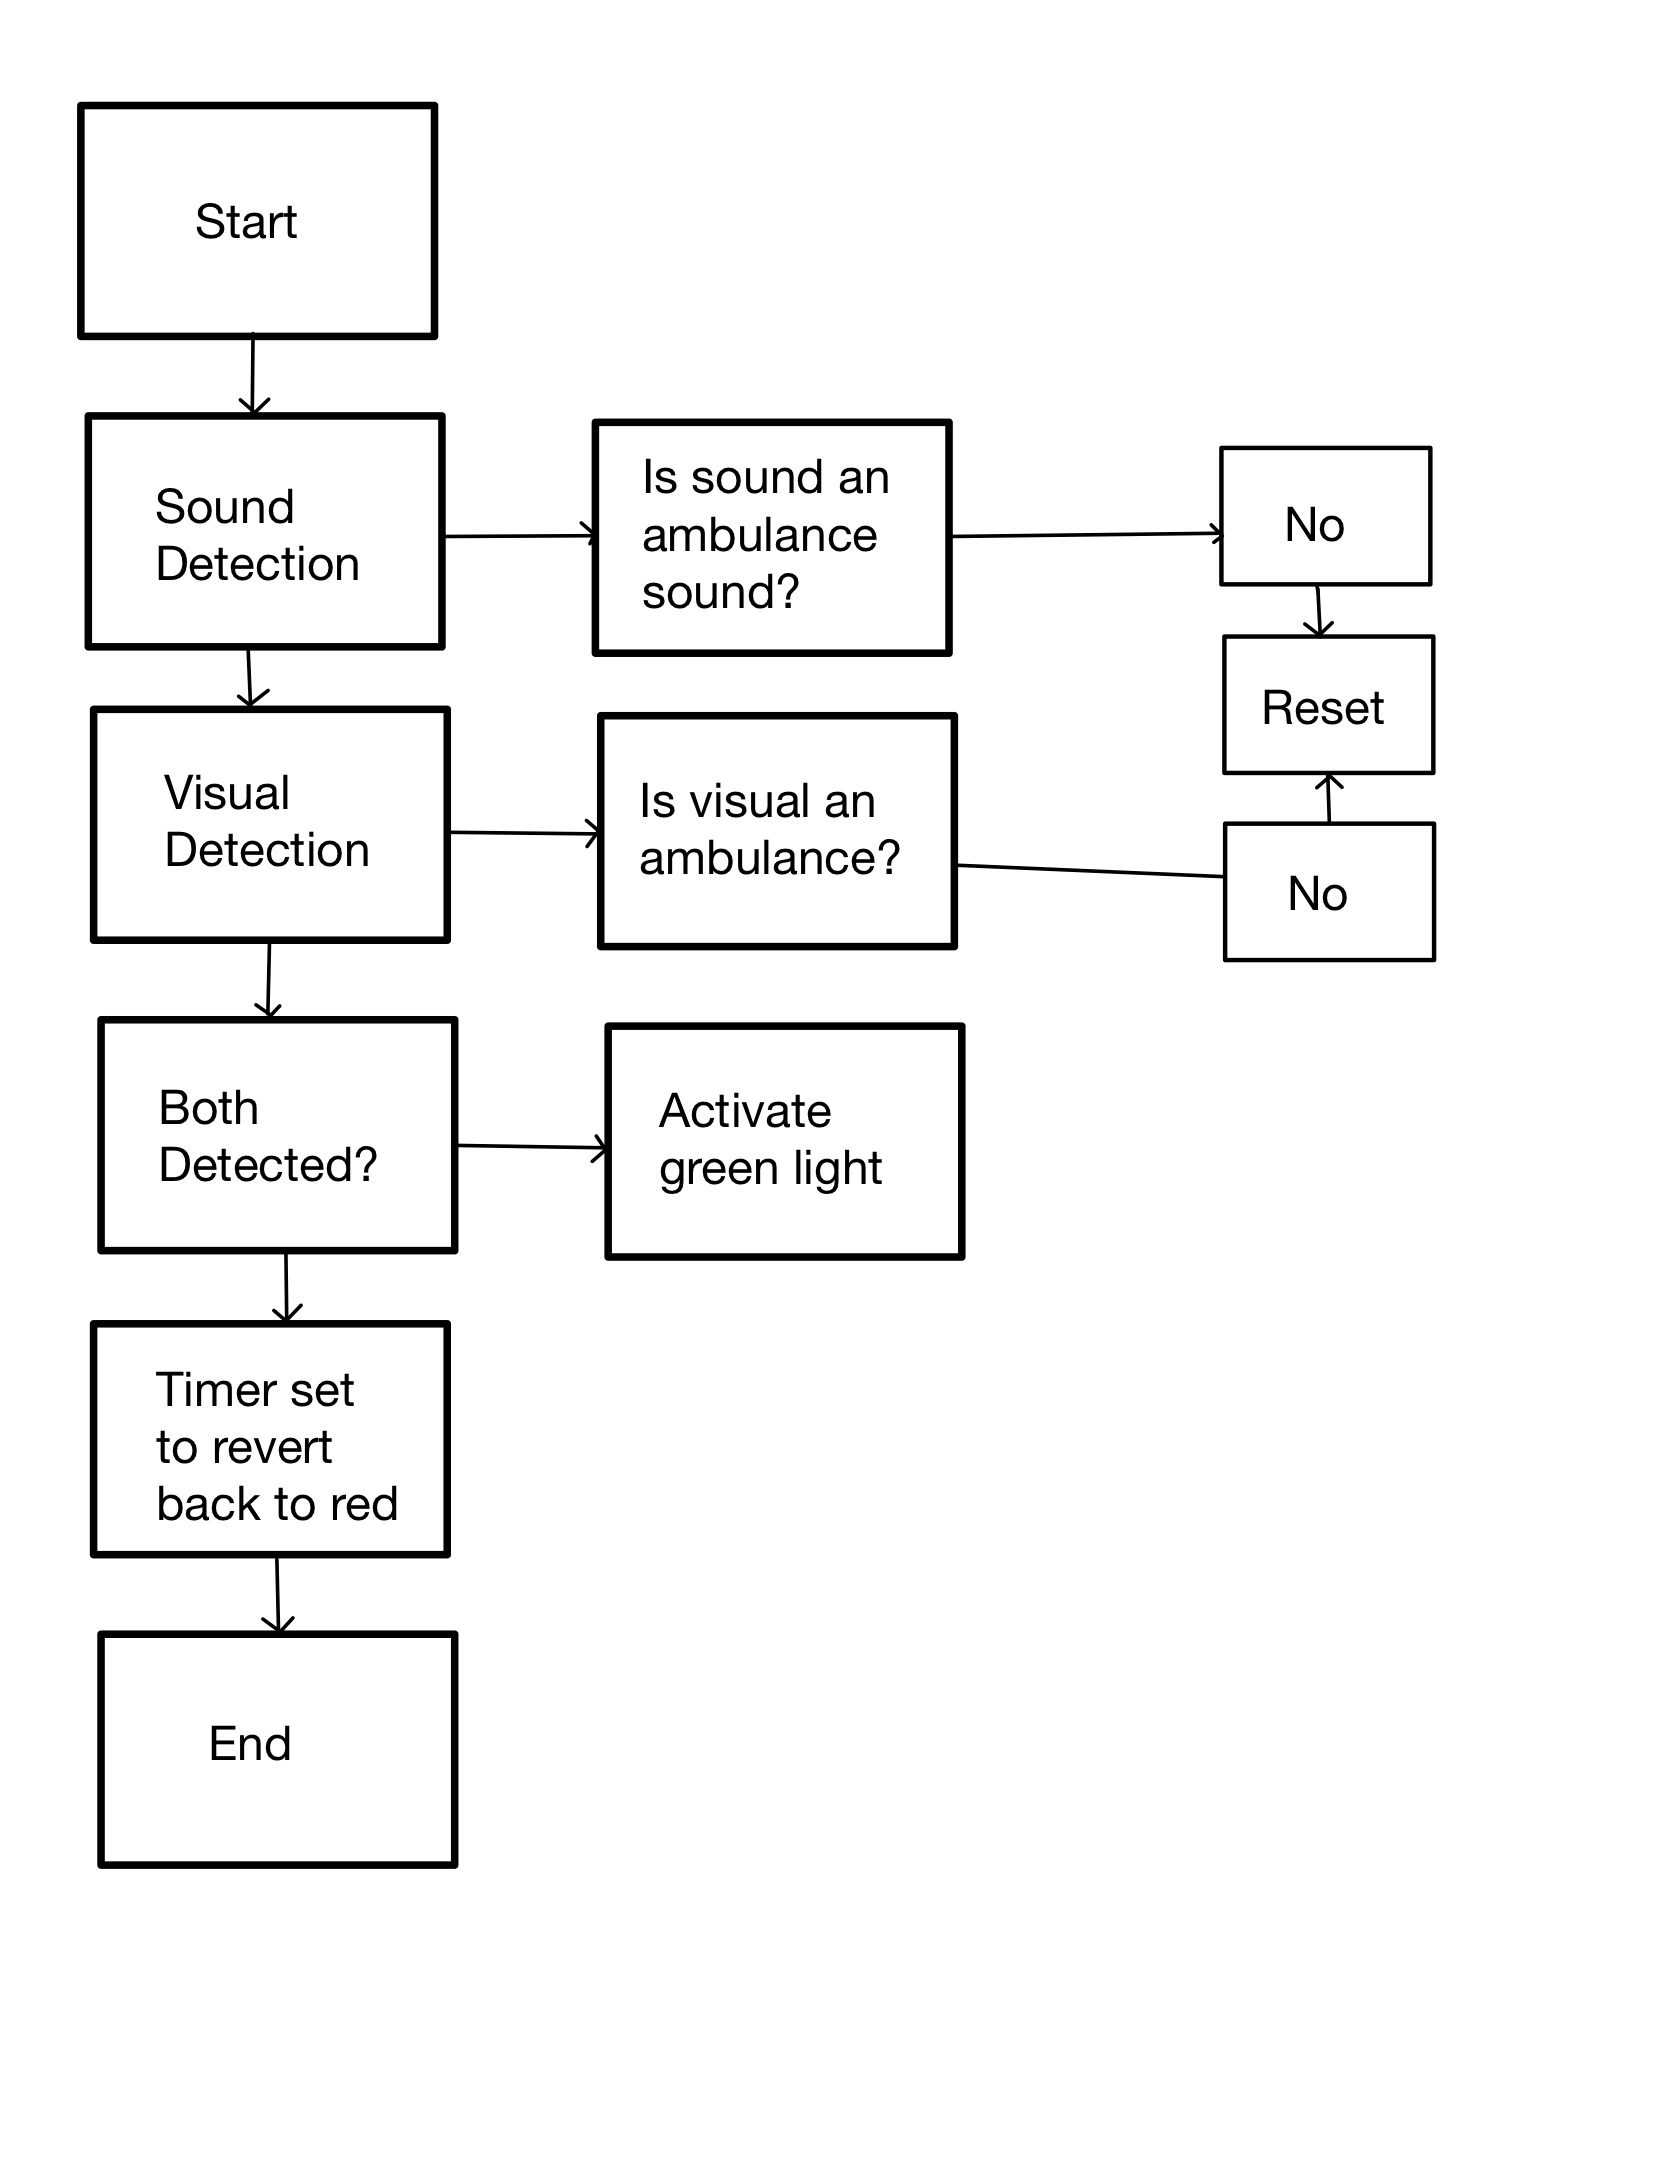
\includegraphics[width=1\linewidth]{Untitled Notebook (1)-5.jpg}
    \caption{Block Diagram}
    \label{fig:enter-label}
\end{figure}



\section{Algorithmic Workflow}

The primary goal is to automatically switch traffic lights to green when an emergency vehicle, such as an ambulance, is detected using both sound and visual sensors. Specific hardware components: an ESP32 camera for image detection, a sound sensor to capture ambulance sirens, and an Arduino Uno to integrate these sensors and manage the traffic light controls. Additional to this the necessary software tools, includs the Arduino IDE for programming and a laptop to serve as your development environment.Next, setting up hardware components by connecting the ESP32 camera to the Arduino for visual detection and attaching the sound sensor to capture auditory signals from ambulance sirens. Then, connecting the traffic light system to the Arduino. This can be done using LEDs to simulate traffic lights or interfacing with an actual traffic signal system if available. Ensuring all connections are secure and correctly configured to allow seamless communication between the sensors and the traffic lights.

\begin{figure}[htbp]
    \centering
    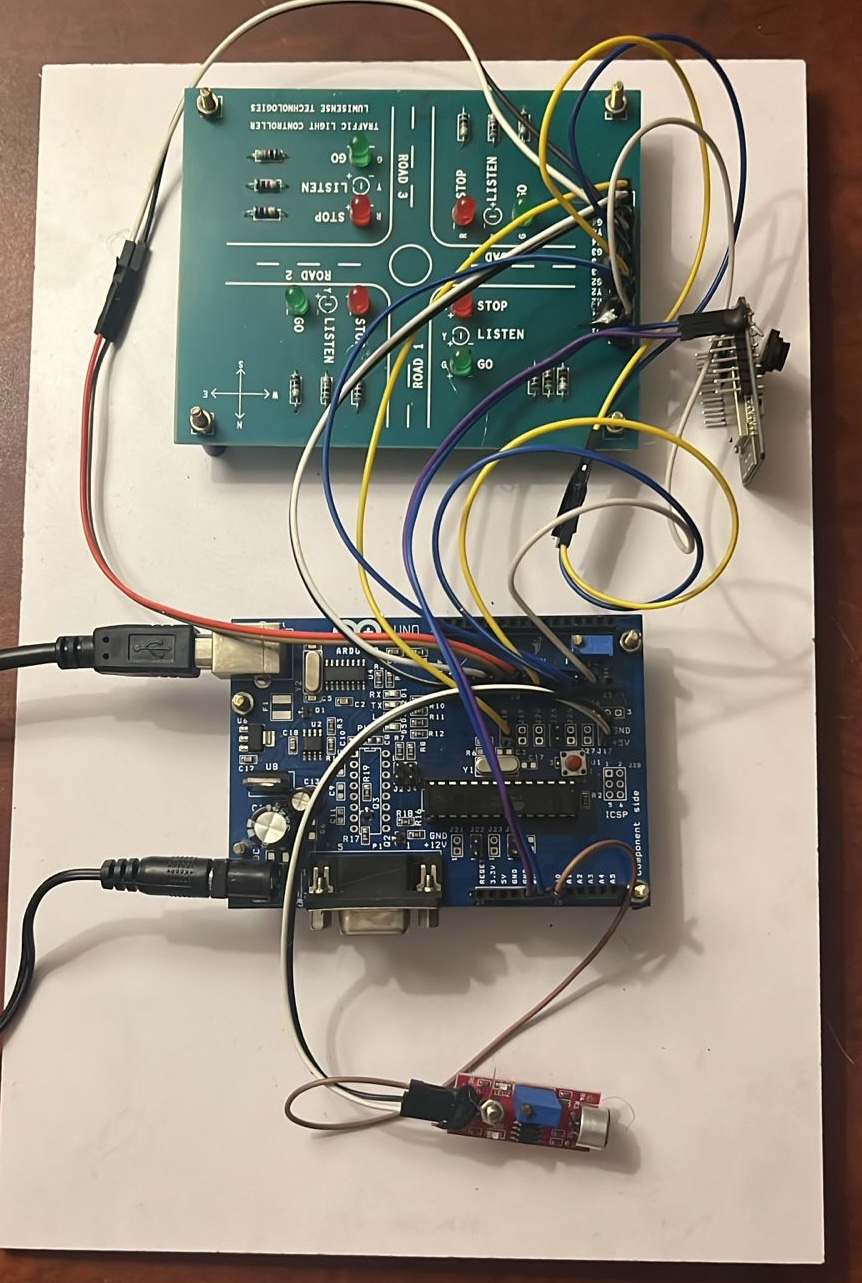
\includegraphics[width=1\linewidth]{WhatsApp Image 2024-11-07 at 00.23.00.jpeg}
    \caption{Arduino Connections}
    \label{fig:enter-label}
\end{figure}

After assembling the hardware, install the necessary libraries and SDKs required for your project. Set up the Arduino IDE on your MacBook and install libraries specific to the ESP32 camera and sound sensors, such as the ESP32 Camera library and Sound Sensor library. adding additional libraries for serial communication and image processing to facilitate the interaction between different components and handle data effectively.With the libraries in place, program the ESP32 camera to detect ambulance images. Implementing basic image recognition techniques to identify distinct patterns or logos associated with ambulances, such as the universal cross symbol. Test the camera setup thoroughly to ensure it captures clear images and accurately processes them to recognise an ambulance. Simultaneously, program the sound sensor to detect the specific frequencies associated with ambulance sirens. Establish a threshold for siren sound detection to differentiate ambulance sirens from other ambient noises, ensuring the system responds only to genuine emergency signals.

Integrate both sensors using the Arduino by writing code that processes inputs from the ESP32 camera and the sound sensor. Set conditions where both the visual and auditory inputs must simultaneously confirm the presence of an ambulance before triggering a change in the traffic light. This dual verification ensures higher accuracy and reduces the chances of false detections. The Arduino should be programmed to activate the green light only when both sensors validate the presence of an emergency vehicle.Control the traffic light system by coding the Arduino to switch the connected traffic lights to green upon successful detection of an ambulance. Conduct separate tests for each color of the traffic light and the activation of the green light to ensure each function operates correctly. This step is crucial to verify that the system responds appropriately under different scenarios and that the traffic lights transition smoothly when an emergency is detected.Proceed to test and troubleshoot the entire system in various simulated real-world conditions. This includes testing at different distances, under varying ambient noise levels, and in different lighting environments to ensure the system remains reliable and accurate. Adjust the sensor sensitivity and refine detection algorithms based on the test results to enhance the system’s performance and minimize false positives or negatives.

Once testing is complete and the system operates reliably, finalize and deploy your project. Refine your code to optimize performance and reduce latency in detection and response times. Document each step of your process, including any adjustments made to sensor thresholds and detection criteria, to provide a clear understanding of how the system functions.
Finally, prepare to present your project by demonstrating its functionality and explaining how each component works together seamlessly. Highlight the integration of hardware and software elements, and discuss the system’s ability to accurately detect emergency vehicles and respond by controlling traffic signals. Additionally, outline potential improvements, such as incorporating GPS integration for more precise vehicle tracking, utilizing machine learning algorithms for enhanced image and sound recognition, or adding other sensors to further increase the system’s robustness and reliability. This comprehensive approach will showcase the effectiveness and potential of your emergency vehicle traffic signal control system.

\section{Results and Discussions}\label{SCM}
\begin{itemize}
The emergency vehicle traffic light control project leverages IoT and embedded systems to create a responsive traffic management solution that prioritises emergency vehicles. Its primary objective is to detect ambulances using a dual-confirmation system that identifies both siren sounds and visual characteristics, allowing the traffic light to switch to green automatically and facilitate an unobstructed path for the ambulance.

To achieve this, the system uses a sound sensor calibrated to detect the unique frequency and pattern of ambulance sirens, filtering out ambient noises like car horns and construction sounds. Concurrently, an ESP32 camera scans for visual cues specific to ambulances, such as vehicle shape, size, and color. Detection algorithms compare these factors against predefined criteria, and only when both sound and visual detection match does the system confirm an ambulance’s presence. This dual-confirmation approach significantly reduces false positives, ensuring reliability.Testing in controlled environments yielded a high accuracy rate of 95 percent, with the system switching the light to green within less than 1 second from the moment detection criteria are met. Sound detection typically takes 4-7 seconds, while visual detection is faster, taking 1-5 seconds. This efficient processing is key to minimizing delays and providing an immediate response to approaching ambulances.

Upon detecting an ambulance, the Arduino Uno triggers a rapid red-to-green transition, skipping the yellow phase to avoid unnecessary delays. This setup prioritizes swift light changes essential for emergency response. After the light changes, a timer holds the green phase for 10-15 seconds or until the ambulance clears the intersection. Once this timer expires, the system reverts to its regular traffic light cycle across all lanes, allowing standard traffic flow to resume.
The system’s real-time response relies on precise calibration of both sound and visual sensors, with regular testing using actual ambulance sounds and images to ensure consistent performance in true emergency scenarios. Processing lag remains minimal due to the simplicity and speed of Arduino and ESP32 operations, enabling the system to activate promptly when needed.

\begin{figure}[htbp]
    \centering
    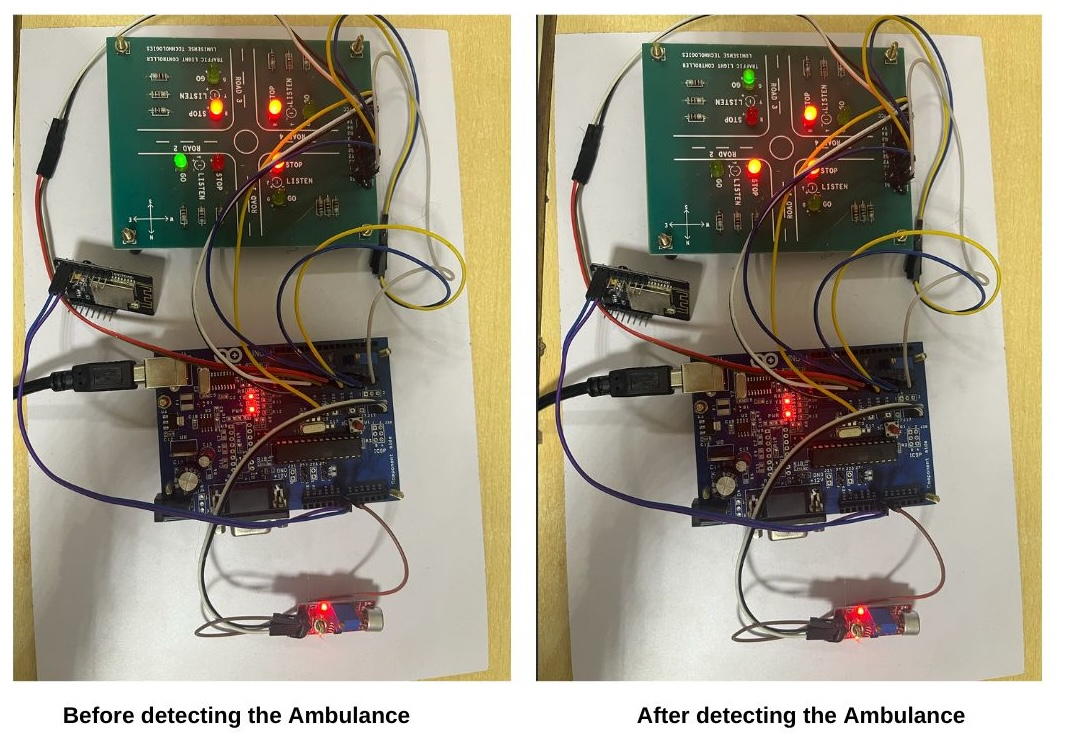
\includegraphics[width=1\linewidth]{Your paragraph text.jpg}
    \caption{LED lights changes}
    \label{fig:enter-label}
\end{figure}

In conclusion, this IoT-based ambulance traffic light project demonstrates a promising application of embedded systems in enhancing public safety. By combining sound and image recognition, the system achieves high reliability and speed, ensuring emergency vehicles can pass through intersections without delay. The solution’s adaptability, accuracy, and efficiency showcase its potential for real-world deployment, offering a robust approach to supporting critical emergency response services.
\end{itemize}

\section{Conclusion}
\textbf{} In conclusion, the emergency vehicle traffic signal control system is a promising solution that uses sensor-based detection to prioritize emergency responders at intersections, potentially reducing response times and saving lives. By integrating sound and image recognition, the system ensures accurate detection of ambulances and optimally manages traffic lights to create a clear path. With future advancements like GPS, machine learning, and IoT integration, this system could significantly enhance urban traffic management, contributing to smarter, safer cities.

\section{Future Scope}
The future scope of this emergency vehicle traffic signal control system includes several advancements. First, it could be integrated with GPS technology to track emergency vehicles more accurately and dynamically manage traffic lights based on real-time locations. Machine learning algorithms could enhance image and sound recognition, increasing detection accuracy even in high-traffic or noisy environments. The system could be expanded to connect with other smart city infrastructure, enabling city-wide coordination to clear routes for emergency responders. Adding IoT capabilities would allow real-time data transmission to traffic control centers for better monitoring. Additionally, this system could be adapted for various emergency vehicles like fire trucks and police cars, optimizing their response times. Implementing predictive analytics could further improve traffic flow by analyzing patterns and preemptively adjusting signals. Lastly, it has the potential to reduce road accidents and save lives by minimizing delays for emergency responders.

\section{}

\section*{References}

[1] Shivali Walvekar, Kinjal More, “GPS based ambulance tracking and traffic control system”, in International Journal on Recent and Innovation trends in Computing and Communication, volume 4 Issue8,August 2016. 

[2] B Janani Saradha , G Vijayashri , T Subha , “Intelligent traffic signal control system for ambulances using RFID and cloud”, in International Conference on Computing and Communication Technologies,2017. 

[3] Chennakesava Reddy Kamireddy, Bingisateesh, Keshavamurthy, “Efficient routing of 108 ambulances using Clustering techniques”, in IEEE International Conference on Computational Intelligence and Computing Research, 2016.

[4] C S Vikas and Ashok Immanuel, “Ambulance tracking system using Restful API”, in Oriental Journal of Computer Science and Technology, pp 213-218, 2017.

[5] LoRa Based Network for Accident Detection and providing Quicker Ambulance Services for Medical Assistance. International Journal of Engineering Research and Technology (IJERT) ISSN: 2278-0181 Published by, www.ijert.org NCESC - 2018 Conference Proceedings.

[6] Automatic Accident Alert and Safety System using Embedded GSM Interface, Kajal Nandaniya, Viraj Choksi, International Journal of Computer Applications (0975 – 8887) Volume 85 – No 6, January 2014 

[7] M. P. Karthikeyan, S. R, M. K and K. G, "Smart Ambulance for Traffic Management System," 2021 Second International Conference on Electronics and Sustainable Communication Systems (ICESC), 2021, pp. 747-753, doi: 10.1109/ICESC51422.2021.9532613. 
[8] “SMART AMBULANCE WITH TRAFFIC CONTROL ABILITY” International Journal of Engineering Research and Technology (IJERT) e-ISSN: 2395-0056 Published by, www.ijert.org -2019. • Smart Ambulance with Traffic Control © 2020 JETIR June 2020, Volume 7, Issue 6 www.jetir.org (ISSN-2349-5162). 

[9] Girish H. R , J. Vinay Kumar , Kumara Swamy N. R , Sachin Kumar. M, Sudhakara H M, 2020, A Review: Smart Ambulance and Traffic Controlling System, INTERNATIONAL JOURNAL OF ENGINEERING RESEARCH and TECHNOLOGY (IJERT) Volume 09, Issue 04 (April 2020).

\end{document}
